\documentclass[a4paper]{article}
\usepackage[utf8]{inputenc}
\usepackage[T1]{fontenc}
\usepackage[polish]{babel}
\usepackage{graphicx}
\usepackage{listings}
\usepackage{float}
\usepackage{geometry}


 \geometry{
 a4paper,
 total={170mm,257mm},
 left=20mm,
 top=20mm,
 }

\graphicspath{ {./images/} }


\begin{document}


\begin{titlepage}
    \begin{center}
        \vspace*{1cm}

        \Huge
        \textbf{Rachunek Macierzowy i Statystyka Wielowymiarowa}

        \Large
        \vspace{0.5cm}
        Raport z zadania 1. - implementacja mnożenia macierzy metodą klasyczną i Bineta

        \vspace{1.5cm}

        \textbf{Wojciech Jasiński, Michał Stefanik}

        \vfill
        \vspace{0.8cm}

        
\includegraphics[width=0.4\textwidth]{agh_logo.jpg}

        Wydział Informatyki\\
        Akademia Górniczo Hutnicza\\
        Kraków\\
        \today

    \end{center}
\end{titlepage}


\section{Pseudokod - ogólna idea}

\begin{verbatim}
    def matmul(A, B, l):
        if rozmiar(A) < 2^l:
            # wykonujemy mnożenie macierzy klasycznie
            return normal_matmul(A, B)
        else:
            # dzielimy macierze na 4 podmacierze
            # wykorzystujemy rekurencyjne wywołanie funkcji matmul dla każdej z podmacierzy
            # podobnie jak w algorytmie Bineta składamy wynik z 4 podmacierzy
            # zwracamy wynik
            return wynik


\end{verbatim}

\section{Pełny kod}

\begin{lstlisting}[language=python]
def binet_normal_mixed_matmul(A, B, l):
    if A.shape[0] <= 2 ** l and A.shape[1] <= 2 ** l and B.shape[1] <= 2 ** l:
        return normal_matmul(A, B)

    A11, A12, A21, A22 = split_matrix(A)
    B11, B12, B21, B22 = split_matrix(B)

    P1 = binet_normal_mixed_matmul(A11, B11, l)
    P2 = binet_normal_mixed_matmul(A12, B21, l)
    P3 = binet_normal_mixed_matmul(A11, B12, l)
    P4 = binet_normal_mixed_matmul(A12, B22, l)
    P5 = binet_normal_mixed_matmul(A21, B11, l)
    P6 = binet_normal_mixed_matmul(A22, B21, l)
    P7 = binet_normal_mixed_matmul(A21, B12, l)
    P8 = binet_normal_mixed_matmul(A22, B22, l)

    C11 = P1 + P2
    C12 = P3 + P4
    C21 = P5 + P6
    C22 = P7 + P8

    return np.vstack(
        (
            np.hstack((C11, C12)),
            np.hstack((C21, C22))
        )
    )

\end{lstlisting}


\section{Wykresy}

\begin{figure}[H]
    \centering
    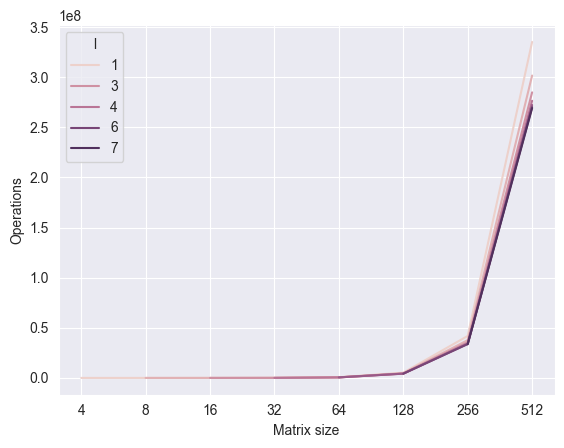
\includegraphics[width=0.7\textwidth]{images/opps.png}
    \caption{Porównanie ilości operacji zmienno przecinkowych podczas mnożenia macierzy w zależności od rozmiaru macierzy i parametru l.}
    \label{fig:opps}
\end{figure}


\begin{figure}[H]
    \centering
    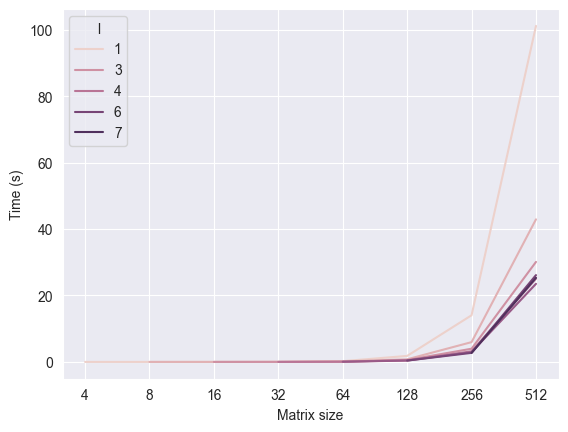
\includegraphics[width=0.7\textwidth]{images/times.png}
    \caption{Porównanie czasów wykonania mnożenia macierzy w zależności od rozmiaru macierzy i parametru l.}
    \label{fig:times}
\end{figure}

\end{document}